\chapter{Metodologia}\label{chap:metodologia}

W~rozdziale opisano podejście badawcze przyjęte w~niniejszej pracy. Opis
obejmuje wybór metody badawczej, strukturę eksperymentu, materiał badawczy,
kryteria oceny, procedurę analizy wyników oraz zasady odtwarzalności. Rozdział
przedstawia sposób przełożenia założeń teoretycznych na kontrolowany plan
badawczy.

\section{Metoda badawcza}\label{sec:metoda-badawcza}

Główny problem badawczy dotyczy wpływu topologii systemu agentowego na jakość
odpowiedzi generowanych na podstawie dokumentów regulacyjnych. Jako podstawową
metodę badawczą przyjęto kontrolowany eksperyment porównawczy, w~którym
warianty systemu przetwarzały ten sam korpus, odpowiadały na identyczny zestaw
pytań i~podlegały ujednoliconej procedurze oceny.

Wybór metody pozwala na izolację sposobu orkiestracji agentów jako jedynej
badanej zmiennej. Zastosowanie odmiennych modeli, indeksów dokumentów lub
zestawów narzędzi uniemożliwiłoby przypisanie różnic w~wynikach wyłącznie
testowanej architekturze. Układ kontrolowany eliminuje wpływ czynników
pobocznych.

Alternatywne metody badawcze zestawiono
w~tabeli~\ref{tab:porownanie-metod-badawczych}. Studium przypadku pojedynczej
architektury uniemożliwia ocenę porównawczą. Analiza teoretyczna pomija wpływ
specyfiki korpusu i~parametrów sterowania na zachowanie modeli językowych.
Z~kolei ankieta ekspercka mierzy subiektywne oczekiwania, a~nie rzeczywiste
parametry działania systemów w~ustandaryzowanych warunkach.

\begin{table}[H]
  \caption{Porównanie metod badawczych}\label{tab:porownanie-metod-badawczych}
  \centering
  \small
  \begin{tabularx}{\textwidth}{@{} p{3.2cm} L L @{}}
    \toprule
    \textbf{Podejście}
    & \textbf{Przydatność}
    & \textbf{Ograniczenie}                                              \\
    \midrule
    Studium przypadku
    & Pozwala szczegółowo opisać jedną architekturę
    & Nie daje podstaw do porównania topologii                           \\
    \addlinespace
    Analiza teoretyczna
    & Ułatwia uporządkowanie pojęć i~oczekiwanych zależności
    & Nie uwzględnia zachowania modelu na konkretnym korpusie            \\
    \addlinespace
    Ankieta ekspercka
    & Może zebrać opinie praktyków lub użytkowników domenowych
    & Mierzy ocenę subiektywną, a~nie przebieg systemu                   \\
    \addlinespace
    Eksperyment porównawczy
    & Umożliwia pomiar jakości i~kosztu w~tych samych warunkach
    & Wymaga ścisłej kontroli konfiguracji i~jednolitego protokołu oceny \\
    \bottomrule
  \end{tabularx}
  \zrodlo{opracowanie własne}
\end{table}

\section{Projekt eksperymentu}\label{sec:projekt-eksperymentu}

Eksperyment polega na porównaniu sześciu topologii agentowych w~identycznym
środowisku zadaniowym. Zmienną różnicującą jest wyłącznie organizacja pracy
systemu, w~tym kolejność kroków, zakres autonomii, podział zadań oraz liczba
wywołań narzędzi.

\subsection{Zmienna niezależna}\label{subsec:zmienna-niezalezna}

Zmienną niezależną jest topologia orkiestracji systemu agentowego. Pojęcie to
oznacza sposób organizacji przepływu informacji, obejmujący m.in. przetwarzanie
sekwencyjne, dekompozycję problemu na podzadania, planowanie działań, wybór
specjalisty na podstawie klasyfikacji pytania oraz iteracyjną modyfikację
kroków w~zależności od wyników pośrednich.

Do eksperymentu wybrano sześć topologii: deterministyczną, planer--wykonawca,
router--specjalista, tablicową, hierarchiczną oraz ReAct. Zestaw dobrano tak,
aby obejmował zarówno architektury jednoagentowe, jak i~wieloagentowe, a~także
różne poziomy autonomii sterowania. Każda architektura musiała pozwalać na
implementację w~jednolitym środowisku bez wprowadzania dodatkowych,
specyficznych narzędzi. Umożliwiło to analizę wpływu orkiestracji na jakość
odpowiedzi.

Tabela~\ref{tab:prownanie-architektur-agentowych} zestawia oba typy architektur
w~kluczowych wymiarach projektowych, stanowiąc punkt odniesienia dla
interpretacji wyników eksperymentu w~\cref{chap:eksperyment-i-wyniki}.

\begin{table}[H]
  \caption{Porównanie architektur agentowych}\label{tab:prownanie-architektur-agentowych}
  \centering
  \small
  \renewcommand{\arraystretch}{1.4}
  \begin{tabularx}{\textwidth}{@{} l L L @{}}
    \toprule
    \textbf{Wymiar}
    & \textbf{Jednoagentowe}
    & \textbf{Wieloagentowe}                                              \\
    \midrule
    Złożoność wdrożenia
    & Niska -- jeden kontekst, jedna instrukcja systemowa,
    jeden punkt awarii
    & Wysoka -- wiele instrukcji systemowych, mechanizmy
    koordynacji, wiele potencjalnych punktów awarii                        \\
    \addlinespace
    Koszt operacyjny
    & Niski -- jedno lub kilka wywołań LLM na pytanie
    & Wysoki -- każdy agent generował osobne wywołania;
    narzut koordynacji zwiększał zużycie
    tokenów~\cite{wang2024survey}                                          \\
    \addlinespace
    Zarządzanie kontekstem
    & Scentralizowane -- wszystkie informacje w~jednym buforze kontekstu;
    ryzyko przekroczenia limitu przy złożonych
    zadaniach~\cite{yao2022react}
    & Rozproszone -- agenci wykorzystywali rozdzielone podzbiory
    informacji; ryzyko utraty danych podczas ich
    przekazywania~\cite{wu2024autogen}                                     \\
    \addlinespace
    Odporność na błąd
    & Błąd w~jednym kroku mógł być skorygowany
    w~kolejnej iteracji pętli
    & Błąd w~węźle nadrzędnym propagował się kaskadowo
    do kolejnych agentów~\cite{wang2024survey}                             \\
    \addlinespace
    Specjalizacja ról
    & Brak -- jeden agent obsługiwał całe zadanie
    & Możliwa -- każdy agent mógł mieć wyspecjalizowaną
    instrukcję, narzędzia i~filtry
    metadanych~\cite{hong2023metagpt}                                      \\
    \addlinespace
    Skalowalność zadań
    & Ograniczona rozmiarem okna kontekstowego
    i~pojemnością pojedynczego modelu
    & Wyższa -- dekompozycja zadania pozwalała przetwarzać
    fragmenty równolegle~\cite{wu2024autogen}                              \\
    \addlinespace
    Przewidywalność
    & Wysoka -- deterministyczny przepływ sterowania zapewnia
    powtarzalność wyników
    & Niższa -- złożoność koordynacji obniża powtarzalność
    odpowiedzi dla identycznych
    zapytań~\cite{wang2024survey}                                          \\
    \addlinespace
    Typowe zastosowanie
    & Pytania wymagające jednego źródła wiedzy,
    systemy z~wymogiem niskich opóźnień
    & Zadania wymagające specjalizacji dziedzinowej,
    złożone przepływy z~wieloma krokami                                    \\
    \bottomrule
  \end{tabularx}
  \zrodlo{opracowanie własne na podstawie literatury}
\end{table}

\subsection{Zmienne zależne}\label{subsec:zmienne-zalezne}

Zmienne zależne obejmują dwa wymiary: jakość odpowiedzi oraz koszt operacyjny.
Ich rozdzielenie wynika z~faktu, że jakość osiągnięta przy dużej liczbie
wywołań modelu stanowi odmienną wartość aplikacyjną niż jakość uzyskana
w~prostszym przebiegu.

Do wymiaru jakości należały: wierność względem pobranych źródeł, poprawność
względem odpowiedzi referencyjnej, zwięzłość oraz trafność pobranych
dokumentów. Do wymiaru operacyjnego należały: opóźnienie, zużycie tokenów,
liczba wywołań narzędzi, liczba iteracji oraz wskaźnik błędów wykonania. Dobór
tych zmiennych wynikał z~metryk omówionych w~części teoretycznej, zwłaszcza
w~kontekście ewaluacji systemów agentowych i~RAG.

\subsection{Warunki kontrolowane}\label{subsec:warunki-kontrolowane}

Utrzymano stałe: model językowy, parametry generacji, korpus dokumentów, indeks
wektorowy, zestaw narzędzi, zbiór pytań, format odpowiedzi oraz procedurę
ewaluacji. Jest to warunek konieczny do zapewnienia porównywalności wyników
i~eliminacji wpływu środowiska testowego na działanie systemu.

Temperaturę generacji ustawiono na zero. Zabieg ten minimalizuje losowość
odpowiedzi modelu i~wariancję między przebiegami, co pozwala przypisać
zaobserwowane różnice bezpośrednio badanym mechanizmom sterowania, a~nie
zmienności LLM.

\begin{table}[H]
  \caption{Zestawienie warunków kontrolowanych}\label{tab:zestawienie-warunkow-kontrolowanych}
  \centering
  \small
  \begin{tabularx}{\textwidth}{@{} p{3.75cm} L @{}}
    \toprule
    \textbf{Element}
    & \textbf{Znaczenie dla porównania}                                    \\
    \midrule
    Model i~parametry
    & Eliminowały wpływ różnej jakości modeli oraz różnej
    losowości odpowiedzi                                                    \\
    \addlinespace
    Korpus dokumentów
    & Zapewniał wspólną podstawę wiedzy dla wszystkich architektur         \\
    \addlinespace
    Indeks wektorowy
    & Utrzymywał jednakowy punkt wyjścia dla etapu wyszukiwania            \\
    \addlinespace
    Zestaw narzędzi
    & Dawał każdej topologii ten sam zakres możliwych działań              \\
    \addlinespace
    Zestaw pytań
    & Pozwalał porównywać odpowiedzi na identycznych przypadkach testowych \\
    \addlinespace
    Protokół ewaluacji
    & Ujednolicał sposób oceny odpowiedzi i~śladów wykonania               \\
    \bottomrule
  \end{tabularx}
  \zrodlo{opracowanie własne}
\end{table}

\subsection{Plan porównawczy}\label{subsec:plan-porownawczy}

Przyjęto pełny plan porównawczy w~układzie zapytanie--architektura. Każde
z~90~pytań zostało obsłużone przez wszystkie sześć topologii, generując łącznie
540~uruchomień. Taki model wewnątrzgrupowy eliminuje wpływ zróżnicowanej
trudności zapytań na wyniki poszczególnych topologii.

Analiza zagregowana definiuje ogólny profil architektury, natomiast analiza
przekrojowa (według poziomu trudności, ubezpieczyciela i~kategorii produktu)
weryfikuje stabilność wyników poszczególnych wariantów przy zmianie warunków
wejściowych.

\section{Materiał badawczy}\label{sec:material-badawczy}

Materiał badawczy składał się z~dwóch części: korpusu dokumentów oraz zestawu
pytań testowych. Korpus stanowił bazę wiedzy dla testowanych systemów,
natomiast zbiór pytań służył do ilościowego pomiaru jakości generowanych
odpowiedzi. Z~uwagi na brak publicznego benchmarku dla polskojęzycznych
dokumentów ubezpieczeniowych, oba komponenty opracowano autorsko.

Korpus obejmował 22~dokumenty ubezpieczeniowe pochodzące od trzech głównych
towarzystw ubezpieczeniowych: ERGO Hestia S.A., Powszechnego Zakładu
Ubezpieczeń S.A. oraz TUiR Warta S.A. Dla każdego ubezpieczyciela uwzględniono
trzy kategorie produktowe: ubezpieczenia komunikacyjne, mieszkaniowe
i~podróżne. W~korpusie znalazły się dwa typy dokumentów: OWU oraz IPID.

Dokumenty ubezpieczeniowe charakteryzują się cechami stanowiącymi wyzwanie dla
architektur RAG i~systemów agentowych: dużą objętością, sformalizowaną
strukturą, obecnością odniesień krzyżowych oraz wymogiem ścisłego rozróżniania
zakresu ochrony, warunków i~wyłączeń. Złożoność korpusu pozwala na wyraźniejsze
uwidocznienie różnic w~skuteczności poszczególnych topologii względem prostych
zbiorów testowych.

Tabela~\ref{tab:zestawienie-korpusu-dokumentow} przedstawia skład korpusu
według ubezpieczycieli.

\begin{table}[H]
  \caption{Zestawienie korpusu dokumentów}\label{tab:zestawienie-korpusu-dokumentow}
  \centering
  \small
  \begin{adjustbox}{max width=0.78\textwidth}
    \begin{tabular}{@{} l c c c @{}}
      \toprule
      \textbf{Ubezpieczyciel}
      & \textbf{Kategorie}
      & \textbf{OWU}
      & \textbf{IPID}                                  \\
      \midrule
      Hestia         & 3                  & 3           & 3           \\
      PZU            & 3                  & 3           & 3           \\
      Warta          & 3                  & 5           & 5           \\
      \midrule
      \textbf{Razem} & \textbf{9}         & \textbf{11} & \textbf{11} \\
      \bottomrule
    \end{tabular}
  \end{adjustbox}
  \zrodlo{opracowanie własne}
\end{table}

Zestaw testowy opracowany na podstawie analizy manualnej dokumentów obejmuje
90~pytań. Do każdego przypisano odpowiedź referencyjną oraz uzasadniający
fragment źródłowy. Umożliwia to zautomatyzowaną ewaluację zgodności wyników
oraz ręczną weryfikację przypadków brzegowych.

Zdefiniowano cztery poziomy trudności. Poziom bardzo prosty testuje podstawową
orientację w~specyfikacji produktu. Poziom prosty wymaga zlokalizowania
pojedynczej informacji bazowej. Poziom złożony narzuca konieczność integracji
warunku, wyjątku lub uzupełniającego fragmentu kontekstu. Z~kolei pytania
bardzo złożone wymuszają syntezę danych z~wielu nieciągłych fragmentów
dokumentu w~celu zbudowania pełnej odpowiedzi.

Zestaw zbalansowano według ubezpieczycieli (po 30~pytań). Trzy główne poziomy
trudności zawierają po 27~pytań, a~poziom bardzo prosty – 9~pytań. Taka
dystrybucja eliminuje ryzyko obciążenia wyników specyfiką pojedynczego dostawcy
lub typu produktu.

\begin{table}[H]
  \caption{Zestawienie rozkładu pytań}\label{tab:zestawienie-rozkladu-pytan}
  \centering
  \small
  \begin{adjustbox}{max width=0.74\textwidth}
    \begin{tabular}{@{} l c c c c @{}}
      \toprule
      \textbf{Poziom trudności}
      & \textbf{Hestia}
      & \textbf{PZU}
      & \textbf{Warta}
      & \textbf{Razem}                                            \\
      \midrule
      Bardzo proste  & 3               & 3           & 3           & 9           \\
      Proste         & 9               & 9           & 9           & 27          \\
      Złożone        & 9               & 9           & 9           & 27          \\
      Bardzo złożone & 9               & 9           & 9           & 27          \\
      \midrule
      \textbf{Razem} & \textbf{30}     & \textbf{30} & \textbf{30} & \textbf{90} \\
      \bottomrule
    \end{tabular}
  \end{adjustbox}
  \zrodlo{opracowanie własne}
\end{table}

Przykłady pytań z~każdego poziomu przedstawia
tabela~\ref{tab:zestawienie-przykladowych-pytan}. Ilustruje ona różnice
w~oczekiwanym nakładzie pracy systemu dla każdej kategorii pytań: od krótkiej
odpowiedzi informacyjnej po odpowiedź wymagającą uwzględnienia warunku
i~wyjątku.

\begin{table}[H]
  \caption{Zestawienie przykładowych pytań}\label{tab:zestawienie-przykladowych-pytan}
  \centering
  \small
  \begin{adjustbox}{max width=0.94\textwidth}
    \begin{tabularx}{0.94\textwidth}{@{} p{2.4cm} L L @{}}
      \toprule
      \textbf{Poziom}
      & \textbf{Pytanie}
      & \textbf{Odpowiedź referencyjna}                                   \\
      \midrule
      Bardzo prosty
      & Na jaki okres zawierana jest standardowo umowa Autocasco z~WARTA?
      & Standardowo umowy AC zawiera się na 12~miesięcy.                  \\
      \addlinespace
      Prosty
      & Na jaki okres może zostać zawarte ubezpieczenie PZU Wojażer?
      & Umowa może zostać zawarta na czas oznaczony od 1~dnia do 1~roku.  \\
      \addlinespace
      Złożony
      & Czy PZU Wojażer obejmuje koszty leczenia spowodowane epidemią?
      & Co do zasady nie, z~wyjątkiem kosztów dotyczących nagłego
      zachorowania na COVID-19, kwarantanny lub izolacji.                  \\
      \addlinespace
      Bardzo złożony
      & Czy w~ubezpieczeniu PZU Wojażer objęte są ochroną koszty
      leczenia chorób przewlekłych?
      & Z~ochrony wyłączone są koszty leczenia chorób przewlekłych,
      z~wyjątkiem zaostrzeń albo powikłań, a~za opłatą dodatkowej
      składki ochrona może zostać rozszerzona do 100\% sumy
      ubezpieczenia.                                                       \\
      \bottomrule
    \end{tabularx}
  \end{adjustbox}
  \zrodlo{opracowanie własne}
\end{table}

\section{Kryteria oceny}\label{sec:kryteria-oceny}

Kryteria oceny zdefiniowano tak, aby uwzględniały zarówno odpowiedź końcową,
jak i~ślad jej generowania. W~systemach agentowych analiza samego wyjścia jest
niewystarczająca do diagnostyki działania. Przykładowo, dwie architektury mogą
wygenerować poprawną odpowiedź, jednak jedna z~nich uzyska ją optymalną ścieżką
wywołań, a~druga wykona operacje nadmiarowe. Z~kolei niska jakość odpowiedzi
może wynikać m.in. z~błędów wyszukiwania, logiki sterującej lub wadliwej
syntezy informacji.

\subsection{Miary ilościowe}\label{subsec:miary-ilosciowe}

Miary ilościowe dobrano spośród metryk omówionych w~rozdziale teoretycznym.
Objęły one dwa obszary: jakość odpowiedzi i~koszt operacyjny. W~obszarze
jakości zastosowano wierność, poprawność względem odpowiedzi referencyjnej,
zwięzłość oraz trafność dokumentów. W~obszarze kosztu uwzględniono opóźnienie,
zużycie tokenów, liczbę wywołań narzędzi, liczbę iteracji oraz błędy wykonania.

Wierność określa stopień pokrycia odpowiedzi pobranymi dokumentami, co jest
kluczowe dla wykrywania halucynacji w~dziedzinie ubezpieczeniowej. Poprawność
względem referencji mierzy trafność merytoryczną niezależnie od formalnej
zgodności z~kontekstem. Zwięzłość weryfikuje użyteczność formatu wyjściowego,
a~trafność dokumentów diagnozuje skuteczność etapu wyszukiwania.

Miary operacyjne charakteryzowały praktyczny koszt działania architektury.
Zużycie tokenów przekładało się bezpośrednio na koszt wywołań modelu,
opóźnienie na czas obsługi żądania, a~liczba narzędzi i~iteracji na złożoność
przebiegu. Wskaźnik błędów wykonania określa niezawodność: wysoka średnia
jakość odpowiedzi traci znaczenie praktyczne w~przypadku wysokiej awaryjności
działania.

Tabela~\ref{tab:zestawienie-metryk-oceny} przedstawia zestawienie wszystkich
zastosowanych miar, ich przedmiot oceny oraz uzasadnienie doboru.

\begin{table}[H]
  \caption{Zestawienie metryk oceny}\label{tab:zestawienie-metryk-oceny}
  \centering
  \small
  \renewcommand{\arraystretch}{1.4}
  \begin{tabularx}{\textwidth}{@{} l l L L @{}}
    \toprule
    \textbf{Wymiar}
    & \textbf{Miara}
    & \textbf{Co oceniała}
    & \textbf{Dlaczego istotna}                                   \\
    \midrule
    \multirow{4}{*}{\centering Jakość}
    & Wierność
    & Czy twierdzenia w~odpowiedzi miały oparcie w~dokumentach
    & Wykrywała halucynacje -- kluczowe w~domenie regulacyjnej    \\
    \addlinespace
    & Poprawność
    & Zgodność z~odpowiedzią referencyjną
    & Oceniała trafność merytoryczną niezależnie od stylu         \\
    \addlinespace
    & Zwięzłość
    & Adekwatność długości do pytania
    & Zbyt rozbudowane odpowiedzi obniżały użyteczność            \\
    \addlinespace
    & Trafność dokumentów
    & Czy pobrane fragmenty były istotne
    & Lokalizowała błąd na etapie wyszukiwania                    \\
    \midrule
    \multirow{4}{*}{\centering Koszt}
    & Zużycie tokenów
    & Łączna liczba tokenów wejściowych i~wyjściowych
    & Bezpośredni wskaźnik kosztu wywołań API                     \\
    \addlinespace
    & Liczba wywołań narzędzi
    & Ile razy architektura odwoływała się do narzędzi
    & Różnicowała architektury o~stałej i~zmiennej liczbie kroków \\
    \addlinespace
    & Opóźnienie
    & Czas od pytania do odpowiedzi końcowej
    & Istotne dla zastosowań produkcyjnych                        \\
    \addlinespace
    & Wskaźnik błędów
    & Odsetek uruchomień zakończonych błędem wykonania
    & Mierzył niezawodność architektury                           \\
    \bottomrule
  \end{tabularx}
  \zrodlo{opracowanie własne}
\end{table}

\subsection{Miary jakościowe}\label{subsec:miary-jakosciowe}

Ocenę ilościową uzupełniono analizą jakościową przebiegów. Jej celem było
ustalenie, w~jaki sposób dana architektura dochodziła do odpowiedzi i~w~którym
miejscu najczęściej dochodziło do spadku jakości. Analizie podlegały pytanie,
pobrane fragmenty, kolejność wywołań narzędzi, ewentualne decyzje sterujące,
odpowiedź końcowa oraz odpowiedź referencyjna.

Analiza jakościowa identyfikuje mocne strony i~ograniczenia topologii
niewidoczne w~wartościach uśrednionych. Przykładowo, architektura o~wysokich
wynikach średnich może generować stały narzut obliczeniowy dla prostych pytań,
a~topologia szybka -- wykazywać niestabilność w~obsłudze zapytań złożonych.

Niepowodzenia klasyfikowano według etapu, na którym powstał problem.
Tabela~\ref{tab:zestawienie-kategorii-bledow} przedstawia przyjętą taksonomię.
Kategorie miały charakter analityczny: pojedynczy przebieg mógł zawierać więcej
niż jeden problem, jednak klasyfikacja według dominującej przyczyny ułatwiała
porównanie architektur.

\begin{table}[H]
  \caption{Zestawienie kategorii błędów}\label{tab:zestawienie-kategorii-bledow}
  \centering
  \small
  \begin{tabularx}{\textwidth}{@{} l L @{}}
    \toprule
    \textbf{Kategoria}
    & \textbf{Opis}                                                        \\
    \midrule
    Błąd wyszukiwania
    & Pobrane fragmenty nie zawierały informacji potrzebnych do odpowiedzi \\
    \addlinespace
    Błąd rozumowania
    & Dowody były dostępne, ale system wyciągał z~nich niepoprawny wniosek \\
    \addlinespace
    Błąd sterowania
    & Topologia wybrała niewłaściwą ścieżkę, rolę, plan albo moment
    zakończenia                                                             \\
    \addlinespace
    Błąd syntezy
    & Odpowiedź końcowa zniekształcała poprawnie pobrane informacje        \\
    \addlinespace
    Nadmiarowy przebieg
    & System wykonywał zbędne kroki, które podnosiły koszt bez poprawy
    jakości                                                                 \\
    \bottomrule
  \end{tabularx}
  \zrodlo{opracowanie własne}
\end{table}

\subsection{Protokół ewaluacji}\label{subsec:protokol-ewaluacji}

Ewaluację odpowiedzi prowadzono dwutorowo. Pierwszy tor stanowiła ocena
automatyczna z~wykorzystaniem modelu językowego w~roli sędziego. Model oceniał
odpowiedzi według zdefiniowanych kryteriów i~zwracał wyniki dla metryk jakości.
Drugi tor stanowiła kontrola autorska, obejmująca przegląd wyników, analizę
przypadków trudnych oraz klasyfikację typów niepowodzeń.

Ewaluacja LLM-as-a-judge automatyzuje pomiar i~skaluje go do 540~uruchomień,
zapewniając jednocześnie determinizm stosowania kryteriów wobec badanych
architektur. Wyniki te służą wyłącznie jako względne porównanie systemów
w~ramach oceny algorytmicznej, nie zaś absolutna weryfikacja poprawności
interpretacji prawnej dokumentów.

W~toku analizy uwzględniono ograniczenia ewaluacji automatycznej: preferencję
wobec długości tekstu, podatność na styl bazowy modelu oraz niedoskonałą
detekcję niuansów dziedzinowych. Wobec tego metryki ilościowe interpretowano
łącznie z~jakościową analizą konkretnych przebiegów wykonania systemu.

\section{Procedura badawcza}\label{sec:procedura-badawcza}

Procedura badawcza definiuje strukturę eksperymentu od preparacji danych do
syntezy wniosków. Kluczowym założeniem jest izolacja etapów generacji, oceny
oraz analizy w~celu wyeliminowania sprzężeń zwrotnych.

\subsection{Etapy eksperymentu}\label{subsec:etapy-eksperymentu}

Proces eksperymentalny obejmuje pięć faz. W~pierwszej przygotowano materiał
badawczy. W~drugiej zdefiniowano warianty architektur. Trzecia faza to
uruchomienie pełnego planu zapytanie--architektura. Faza czwarta obejmuje
ewaluację. Piąta faza to wielowymiarowa analiza wyników (ilościowa, jakościowa
oraz produkcyjna).

\begin{figure}[H]
  \caption{Etapy eksperymentu}\label{fig:etapy-eksperymentu}
  \centering
  \begin{adjustbox}{max width=\textwidth}
    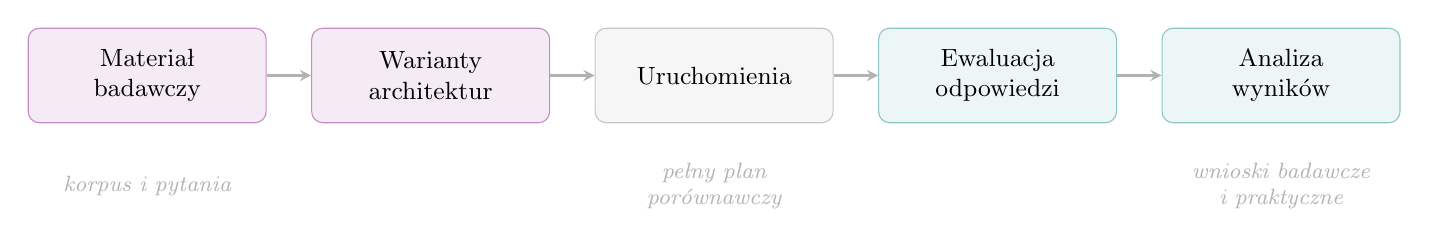
\begin{tikzpicture}[
        stepbox/.style={rectangle, draw, rounded corners=4pt,
          minimum width=2.8cm, minimum height=1.2cm,
          text width=2.6cm, align=center, text centered,
          inner sep=6pt, font=\small,
        fill=gray!7, draw=gray!45},
        arrow/.style={->, >=stealth, draw=gray!60, thick},
        lab/.style={font=\footnotesize\itshape, text=gray!60,
        align=center, text width=2.6cm}
      ]
      \node[stepbox, fill=violet!8, draw=violet!45] (s1) at (0,   0)
      {Materiał\\badawczy};
      \node[stepbox, fill=violet!8, draw=violet!45] (s2) at (3.6, 0)
      {Warianty\\architektur};
      \node[stepbox]                                (s3) at (7.2, 0)
      {Uruchomienia};
      \node[stepbox, fill=teal!7, draw=teal!45]     (s4) at (10.8,0)
      {Ewaluacja\\odpowiedzi};
      \node[stepbox, fill=teal!7, draw=teal!45]     (s5) at (14.4,0)
      {Analiza\\wyników};
      \draw[arrow] (s1) -- (s2);
      \draw[arrow] (s2) -- (s3);
      \draw[arrow] (s3) -- (s4);
      \draw[arrow] (s4) -- (s5);
      \node[lab] at (0,   -1.4) {korpus i~pytania};
      \node[lab] at (7.2, -1.4) {pełny plan\\porównawczy};
      \node[lab] at (14.4,-1.4) {wnioski badawcze\\i~praktyczne};
    \end{tikzpicture}
  \end{adjustbox}
  \zrodlo{opracowanie własne}
\end{figure}

Izolacja etapu ewaluacji zapobiega przekazywaniu informacji zwrotnej do
architektur generujących. Gwarantuje to, że każdy zarejestrowany przebieg jest
niezależnym i~obiektywnym wynikiem działania badanej topologii na przypisanym
pytaniu.

\subsection{Analiza ilościowa}\label{subsec:analiza-ilosciowa}

Analiza ilościowa realizowana jest dwupoziomowo. Poziom zagregowany obejmuje
wskaźniki uśrednione: jakość, koszt, opóźnienie, zużycie tokenów i~liczbę
błędów, definiujące ogólny profil efektywności każdej konfiguracji.

Poziom przekrojowy analizuje wyniki m.in. w~zależności od stopnia trudności
zapytania. Pozwala to zweryfikować korelację między złożonością topologii a~jej
skutecznością w~zadaniach wieloetapowych. Analiza przekrojowa eliminuje ponadto
ryzyko zaburzenia wyników przez lokalne ekstrema trudności w~poszczególnych
fragmentach korpusu.

Wnioski ilościowe są ograniczone do testowanej specyfiki i~nie stanowią
uniwersalnego benchmarku systemów agentowych. Ich zasadniczym celem jest
zmapowanie relacji między jakością a~kosztem na poziomie poszczególnych
topologii.

\subsection{Analiza jakościowa}\label{subsec:analiza-jakosciowa}

Analiza jakościowa koncentruje się na wybranych, brzegowych śladach wykonania:
przypadkach o~skrajnie niskiej ocenie, przerwaniach z~błędem oraz anomaliach
kosztowych. W~celu identyfikacji przyczyn niepowodzenia odtwarza się pełny ciąg
zdarzeń: od rozpoznania intencji do syntezy końcowej.

Badanie to ma na celu identyfikację wzorców błędów. Przykładowo,
w~architekturze router--specjalista weryfikuje się trafność klasyfikacji
zapytania; dla wariantów iteracyjnych -- celowość powtarzania kroków; dla
topologii zdecentralizowanych -- stabilność utrzymania danych w~toku przepływu
informacji.

Wyniki oceny jakościowej stanowią niezbędny kontekst dla metryk ilościowych,
umożliwiając odróżnienie architektur o~zbliżonej średniej, lecz odmiennych
klasach dominujących awarii.

\subsection{Perspektywa produkcyjna}\label{subsec:perspektywa-produkcyjna}

Ostatni wymiar analizy przekłada wyniki z~warunków kontrolowanych na środowisko
produkcyjne. Zdefiniowano w~nim granice uzasadnionej złożoności orkiestracji
oraz wskaźniki stabilności wdrożeniowej.

Wdrożenie komercyjne wymaga uwzględnienia przewidywalności, kosztu obsługi
i~ciągłości działania. Wobec tego wnioski z~eksperymentu przyjmują formę
rekomendacji wielokryterialnych, dostosowujących wybór architektury do wymagań
wierności, budżetu operacyjnego oraz przewidywanego stopnia złożoności systemu
produkcyjnego.

\section{Odtwarzalność}\label{sec:odtwarzalnosc}

Odtwarzalność jest jednym z~warunków wiarygodności eksperymentu. W~niniejszej
pracy miała ona istotne znaczenie, ponieważ badanie dotyczyło systemów opartych
na dużych modelach językowych, których zachowanie zależy od konfiguracji
modelu, wersji usług, sposobu przygotowania danych oraz treści promptów.

Odtwarzalność środowiska badawczego zabezpieczono przez pełną archiwizację
kodu, konfiguracji LLM, korpusów oraz logów ewaluacyjnych w~postaci zwartego
zestawu artefaktów. Takie ujęcie ustanawia referencyjny punkt odniesienia do
powtórnej weryfikacji obliczeń.

Z~racji zależności od zewnętrznych platform udostępniających modele przez API,
absolutna niezmienność wyników na poziomie generacji tokenów nie jest
gwarantowana. Jako środki zaradcze wprowadzono logowanie parametrów i~wersji
modeli w~repozytorium oraz udostępniono pełny zapis przebiegów, na których
bezpośrednio oparto wnioski badawcze.